{
{\sffamily Vi giver nu en kort vurdering af de enkelte dele, som er
blevet udviklet.
}

\subsection{Udtrækning af regioner}
Vores udtrækning af regioner er på ingen måde perfekt. Det er har dog
ikke været et mål i sig selv, at lave decideret god udtrækning af
regioner, blot noget der virker. Når udtrækningen af regioner ikke er
særlig sofistikeret, kan vi senere komme til at tage nogle dårlige valg,
da vores metoder, som vurderer regioner, antager, at den kun modtager
interessante regioner i billedet.

\subsection{Vurdering af regioner}
Det er nævnt helt fra start, at problemet at afgøre, om noget er
interessant i et billede, er et utroligt følsomt område. Med den
udtrækning af regioner vi har, kan vi ikke vurdere regionerne på andet
end deres størrelse og masse. Hvis man begynder at vurdere regionerne på
andre områder, såsom deres massemidtpunkt eller fordeling, tager vi
beslutninger som egentlig vedrører, om regionen ligger godt i et givet
snit.

Vores naive vurdering af regioner, fungerer sådan set fint nok, givet
tilpas simple billeder eller bedre udtrækning af regioner. Metoden
mangler dog en egenskab, lignende den fra den udvidede vurdering, hvor
man også kigger på regionens udstrækning i billedet, således at man ikke
udvælger regioner, hvor store dele af massen ligger langt væk fra
snittet. Dette indfører dog et nyt spørgsmål, for hvornår ligger noget
egentlig langt væk fra snittet?

Den udvidede metode tillader, til en vis grad, mindre fejl i udvælgelsen
af regioner, end den naive vurdering, da kravene til er mere præcist
defineret. Man skal dog kraftigt overveje, hvilket størrelse gitter der
bruges, til at approksimere regionerne, da dette har markant indflydelse
på køretiden.

De to metoder søger dog at udvælge vidt forskellige former for regioner.
Den naive finder de der ligger op ad snittet, mens den udvidede finder
dem som centrerer sig på snittet. Det er derfor oplagt at kombinere
metoderne, således at vi vælger begge typer regioner. Udvælgelsen af
regioner er dog stadig binær --- enten godtages en region, eller også
gør den ikke --- og deri ligger deres største svaghed. Vi kan nemlig
ikke umiddelbart sammenligne to godkendte regioner, for at afgøre
hvilken der ligger bedst i snittet.

\subsection{Databaseskema}
Resultaterne, der gemmes i databasen, er kun de regioner som er blevet
udvalgt til at ligge i snittet. Dette giver god mening, da det i sandhed
kun er dem, som vi anser som interessante. Der kastes dog en del
information væk angående analysen, da der ikke gemmes noget tal for hvor
mange regioner der er blevet sorteret fra.

\subsection{Datasæt}
Vores korpus kunne godt være bedre organiseret, selvom vi dog skal være
glade for overhovedet at have adgang til al den metadata, som vi har
fået fra wga.hu's kommaseparerede fil.

\begin{figure}[!h]
    \centering
    \subfloat[Original]{
        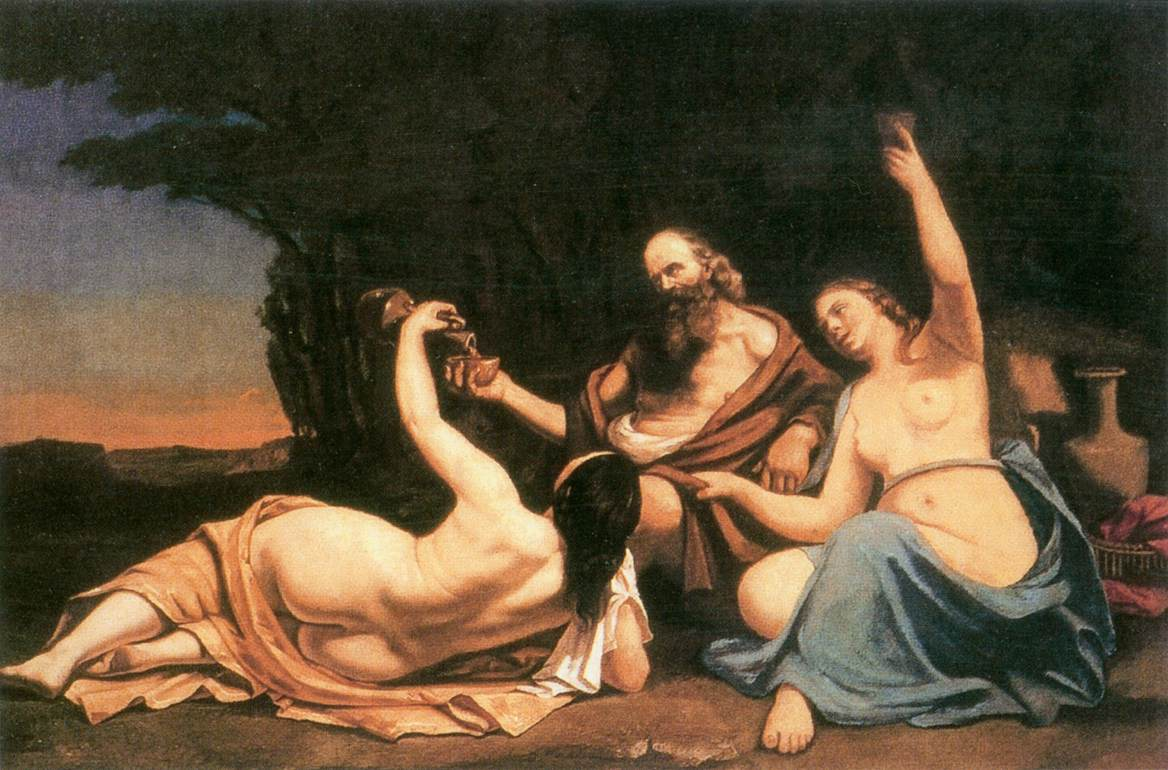
\includegraphics[angle=0,width=0.8\textwidth]{afsnit/fremtidigt_arbejde/billeder/courb101.jpg}
        \label{fucked_original}
    }\\
    \subfloat[Billede sammensat af flere billeder]{
        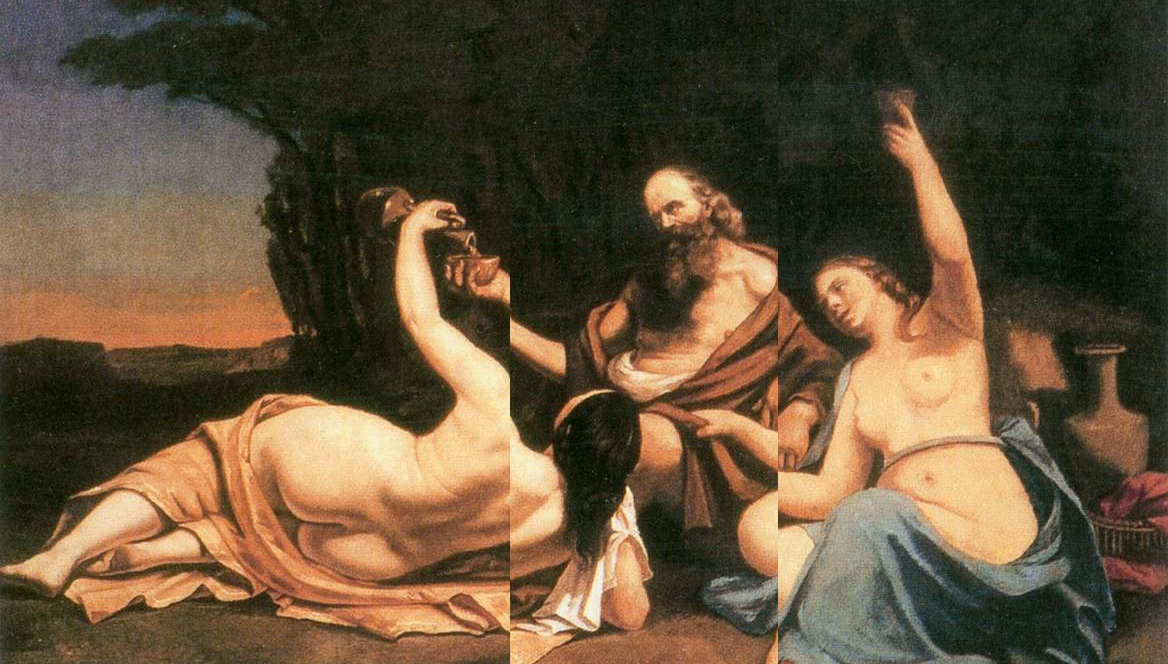
\includegraphics[angle=0,width=0.8\textwidth]{afsnit/fremtidigt_arbejde/billeder/fucked_painting.png}
        \label{fucked_up_painting}
    }
    \caption[]{Problemer der kan opstå ved sammensætning af flere
    billeder. Bemærk, at det sammensatte billede er blevet beskåret,
    hvilket sår tvivl om målingers præcision i billedet.}
    \label{fucked_sammensaetning}
\end{figure}

En bedre parser kunne måske gøre, at billeder, som er blevet delt op,
blev samlet til ét billede når vi hentede dette. Opgaven at samle to
eller flere billeder til et, kan dog også vise sig at være en
kompliceret opgave, da vi ikke ved, om de enkelte billeder engang har
været del af det samme digitale billede, som blot er delt op. Hvis
billederne bare sættes sammen, kan vi have, at det færdige billede
bliver sat skævt sammen, pga. forskelligt perspektiv i billederne, som
der er vist et eksempel på i figur \ref{fucked_up_painting}. Der findes
helt sikkert metoder til at løse problemet i figur
\ref{fucked_up_painting}, men man vil sikkert komme ud for problemer med
beskæring af det sammensatte billede.

At afgøre, hvorvidt et billede er et udsnit af et større billede, vil
enten kræve en meget omfattende parser eller en omstrukturering af data
i wga.hu's kommaseparerede fil, så det blev klart indikeret, hvor et
billede hører til.

}

% vim: set tw=72 spell spelllang=da:
